\documentclass[11pt, a4paper]{article}
%\usepackage[danish]{babel}
\usepackage{amsmath}
\usepackage[utf8]{inputenc}
%\usepackage{xfrac}
\usepackage{amsfonts}
\usepackage{amssymb}
\usepackage{tikz}
\usepackage{array}
\usepackage{cancel}
\usepackage{ulem}
\usepackage{graphicx}
\usepackage[a4paper]{geometry}
\usepackage{gauss}
%\usepackage{mathtools}
\usepackage{amsmath}
\usepackage{lastpage}
\usepackage{fancyhdr}
\usepackage{multirow}
\usepackage{listings}
\setlength{\headheight}{15.2pt}
\pagestyle{fancy}
\fancyhf{}
\lhead{Mads Anthony, MANA} %husk denne
\rhead{Side\ \thepage\ af\ \pageref{LastPage}} %husk 2 builds for dette!
%\usepackage[ansinew]{inputenc} 
\usepackage{enumerate}
%dot2tex loads
\usetikzlibrary{shapes}
\begin{document}
\author{Mads Anthony}
\section{Experiments}
\subsection{Setup}

\subsubsection{Microscopic Oscilliations HyperNEAT (MiO-HyperNEAT)}
The general idea with this method is to try and mimic the oscillation that happens on the microscopic level of the brain and use that to modularize the network. As mentioned earlier, the microscopic oscillations (MiO) is the firing patterns that take place for each neuron. To mimic this, MiO-HyperNEAT uses HyperNEAT together with SUPG to evolve oscillations for each hidden neuron placed on the substrate. 
\\
\\
Along with the oscillation evolved for each hidden neuron the network on the substrate has an extra output that generate a \textit{Master Frequency}. The master frequency, isn't evolved using a SUPG, but is instead generated as a normal output (that if necessary can be modulated onto some pre-defined function - ex. sine function). The idea with the master frequency is to generate a frequency that is dependent on the environment, whereas the neuron oscillations only are determined by their position on the substrate.
\\
\\
Each hidden neuron then compare their oscillations with the master frequency, and if they are in synchrony they are enabled, and if not - they are disabled. One reason for this, is to let Hyper-NEAT try to discover frequencies that make part of the network be active at different times. Another reasons is that research (as mentioned earlier) points to certain oscillations be in synchrony for different task.
\\
\\
Since the total number of ways the hidden neurons can be active/disabled is $ 2^n $ it could in theory mean that Hyper-NEAT could discover $ 2^n $ modules - where $ n $ is the number of hidden neurons. A setup of the method can be seen in figure (x).
\begin{figure}[!ht]
\centering
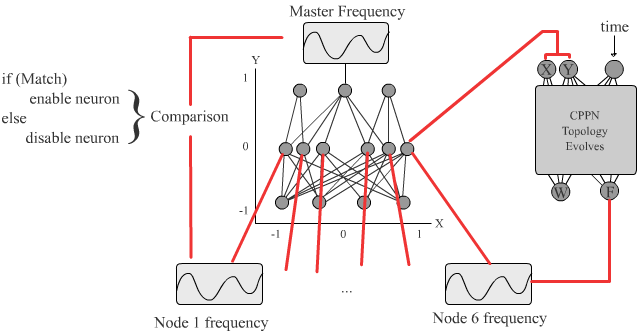
\includegraphics[scale=0.5]{MiO-HyperNEAT}
\caption{}
\end{figure}
\subsubsection{MaO-HyperNEAT}
\subsection{Experiment 1 - Recognizing time patterns}
\begin{center}
    \begin{tabular}{ | p{4cm} | l | l | l |}
    \hline
    Function & Image1 & Image2 & Error term ($ r^2 $) \\ \hline
    \begin{equation} f(x) =
    \begin{cases}
      0, & \text{if}\ x<0.5 \\
      1, & \text{otherwise}
    \end{cases} \nonumber \end{equation} &  \raisebox{-1\height}{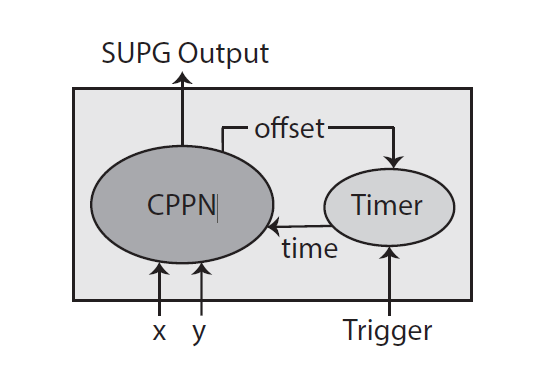
\includegraphics[scale=0.2]{SUPG}} &
\raisebox{-1\height}{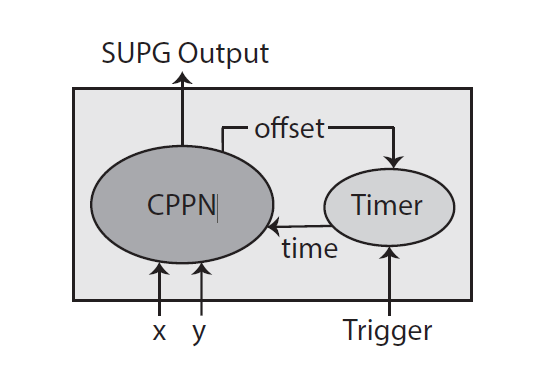
\includegraphics[scale=0.2]{SUPG}} &  
0.9
\\
    \hline
   \begin{equation} f(x) = sin(x) \nonumber \end{equation}  &
    &  &  \\
   \hline
   \begin{equation} f(x) = 3 \cdot sin(x+2) \nonumber \end{equation}  & & &  \\
   \hline
    \end{tabular}
\end{center}
\subsection{Experiment 2 - Timely split task (Simple domain)}
\subsubsection{Domain}
\subsubsection{Results}
\subsection{Experiment 3 - Environment split task}
\subsubsection{Domain}
\subsubsection{Results}
\end{document}